\documentclass[11pt]{article}

% --- Silnik: xelatex ---
\usepackage{fontspec}
\setmainfont{DejaVu Serif}[Scale=0.94]
\setsansfont{DejaVu Sans}[Scale=0.94]
\setmonofont{DejaVu Sans Mono}[Scale=0.86]

\usepackage{amssymb}
\usepackage[a4paper,margin=2.3cm]{geometry}
\usepackage{xcolor}
\usepackage{titlesec}
\usepackage{enumitem}
\usepackage{booktabs}
\usepackage{tabularx}
\usepackage{array}
\usepackage{tikz}

\definecolor{navy}{RGB}{19,40,82}
\definecolor{rulegrey}{RGB}{180,190,205}
\definecolor{accent}{RGB}{0,110,90}

\emergencystretch=3em
\hbadness=2500

\titleformat{\section}{\Large\bfseries\sffamily\color{navy}}{}{0pt}{}
\titleformat{\subsection}{\large\bfseries\sffamily\color{navy}}{}{0pt}{}
\titleformat{\subsubsection}{\normalsize\bfseries\sffamily\color{navy}}{}{0pt}{}
\titlespacing*{\section}{0pt}{1.25em}{0.4em}
\titlespacing*{\subsection}{0pt}{0.85em}{0.2em}
\titlespacing*{\subsubsection}{0pt}{0.6em}{0.15em}

\setlength{\parindent}{0pt}
\setlength{\parskip}{0.5em}
\setlist[itemize]{leftmargin=1.3em,itemsep=0.12em,topsep=0.2em}
\setlist[enumerate]{leftmargin=1.5em,itemsep=0.12em,topsep=0.2em}

\newcommand{\ra}{$\rightarrow$}
\newcommand{\key}[1]{\textbf{\color{navy}#1}}

\begin{document}

% ====== TYTUL ======
{\sffamily\bfseries\color{navy}\LARGE Projekt: Cyfrowy bliźniak i testbench diagnostyczny ładowarek AC}\\[3pt]
{\sffamily\large\color{navy} Model-based diagnostyka, weryfikacja licznika i raporty do producenta}\\[5pt]
{\color{rulegrey}\rule{\linewidth}{1pt}}\\[3pt]
{\sffamily\small Dawid Cekała \quad$\cdot$\quad zadanie rekrutacyjne AMPERE POINT --- część 2 \quad$\cdot$\quad wersja 3 \quad$\cdot$\quad 16 czerwca 2026}

\vspace{0.7em}

% ====== TLDR ======
\section{Streszczenie (w jednym oddechu)}

Buduję \key{cyfrowego bliźniaka} ładowarki AC w Simulink/Simscape: model „idealnej, zgodnej z normą'' ładowarki, który służy jako \key{złoty wzorzec}. Do tego \key{emulator samochodu} ze scenariuszami i \key{wstrzykiwaniem usterek}, który prowadzi zarówno wzorzec, jak i (opcjonalnie, przez tani adapter) realną ładowarkę. \key{Komparator} porównuje zachowania i wystawia werdykt pass/fail oraz \key{twardy, powtarzalny raport do producenta w Chinach}. Całość projektuję i demonstruję w symulacji --- bez kapitału, w ok. 40~h. To zamienia obecny, podstawowy „tester wallboxów'', który firma rozdaje w gratisie, w realne narzędzie diagnostyki i kontroli jakości, dopasowane do modelu „OEM na sterydach''.

% ====== PRIMER ======
\section{1. Najpierw zrozummy ładowarkę AC (od zera)}

To moje pierwsze zetknięcie z tymi ładowarkami, więc najpierw układam fundament --- bez tego koncepcja nie ma sensu.

\subsection{1.1. Ładowarka AC to „inteligentny włącznik'', nie prostownik}

Bateria auta przyjmuje prąd stały (DC). Z gniazda płynie prąd przemienny (AC). Zamiana AC\ra{}DC (prostownik) siedzi \key{w samochodzie} (ładowarka pokładowa). Wallbox czy ładowarka przenośna \key{nie zamieniają prądu} --- one tylko bezpiecznie podają AC i \key{dogadują się z autem}, ile prądu może popłynąć. Wniosek dla projektu: cała „inteligencja'' ładowarki AC to \key{sygnalizacja, sterowanie i zabezpieczenia} --- i to właśnie da się modelować i testować od zewnątrz, bez zaglądania do środka.

\subsection{1.2. Rozmowa ładowarki z autem --- Control Pilot (handshake)}

Komunikacja idzie jedną żyłą sygnałową --- \key{Control Pilot (CP)}. Ładowarka podaje na nią napięcie, a auto swoimi rezystorami „ściąga'' je do konkretnych poziomów; każdy poziom to inny \key{stan}. Gdy auto jest gotowe, ładowarka nadaje na CP \key{sygnał PWM} (prostokątny, 1~kHz), którego \key{wypełnienie} koduje maksymalny prąd. To jest serce normy \key{IEC 61851} i serce mojego modelu.

\begin{center}
\begin{tabularx}{0.92\linewidth}{@{}c c X@{}}
\toprule
\textbf{Stan} & \textbf{Napięcie CP} & \textbf{Znaczenie} \\
\midrule
A & $+12$~V & brak auta (spoczynek) \\
B & $+9$~V & auto podłączone, jeszcze nie ładuje \\
C & $+6$~V & auto ładuje \\
D & $+3$~V & ładowanie z wymuszoną wentylacją (rzadkie) \\
E / F & $0$ / $-12$~V & błąd / ładowarka niedostępna \\
\bottomrule
\end{tabularx}
\end{center}

Kodowanie prądu: \key{prąd [A] = wypełnienie [\%] $\times$ 0,6} (w zakresie 10--85\%). Np. 25\% \ra{} 15~A, 50\% \ra{} 30~A, ok. 53\% \ra{} 32~A. Druga żyła, \key{Proximity Pilot (PP)}, mówi rezystorem, jaki kabel jest podłączony i ile prądu wytrzyma.

\subsection{1.3. Licznik energii --- i dlaczego jego dokładność jest krytyczna}

Ładowarki AMPERE POINT mają \key{niezerowalny licznik energii (kWh)}. Ze strony firmy: to filar oferty dla flot --- pracownik ładuje auto służbowe w domu, a firma rozlicza koszt na podstawie odczytu licznika (seria Q dodaje historię i eksport w aplikacji Tuya). \key{Jeśli licznik myli się o kilka procent, klient dostaje złe faktury} --- a to spór i utrata zaufania. Dokładność licznika to więc nie detal, tylko realna wartość biznesowa, którą da się i warto testować.

\subsection{1.4. DLB --- równoważenie mocy (gdzie najczęściej coś „nie gra'')}

Wallbox PRIME ma \key{Dynamic Load Balancing (DLB)} do 4 stacji: rozdziela dostępną moc tak, by nie wybić bezpiecznika. To klasyczne miejsce na błędy: ładowarka musi \key{w porę} (norma: w kilka sekund) zmniejszyć prąd, gdy w domu rośnie inne obciążenie, i ponownie go zwiększyć, gdy auto się odłączy. Wolna albo błędna reakcja = wybity bezpiecznik lub niepotrzebnie wolne ładowanie.

\subsection{1.5. Mapa awarii --- gdzie realnie powstają problemy}

\begin{itemize}
  \item \key{Handshake CP:} zły poziom stanu, brak diody (auto „udaje'' kabel), nieczyste przejścia B\ra{}C.
  \item \key{Prąd:} ładowarka oferuje złe wypełnienie PWM \ra{} za wolno albo ponad bezpiecznik.
  \item \key{Reakcja w czasie:} zbyt wolna odpowiedź na polecenie zmniejszenia prądu (DLB).
  \item \key{Licznik:} przekłamanie kWh \ra{} złe rozliczenia floty.
  \item \key{Bezpieczeństwo:} brak reakcji na usterkę (zwarcie CP, brak diody) zamiast odcięcia.
  \item \key{Regresje firmware:} nowy firmware od producenta „naprawia jedno, psuje drugie''.
\end{itemize}

% ====== REALIA FIRMY ======
\section{2. Realia AMPERE POINT --- i co z nich wynika}

Zebrane z ich strony i z rozmowy --- to fundament dopasowania projektu:

\begin{itemize}
  \item \key{„OEM na sterydach''.} Zamawiają gotowy sprzęt (z Azji), magazynują w Polsce (Tuchom k.\ Gdańska, wysyłka 48~h), testują, wdrażają i sprzedają bezpośrednio. Hasło ze strony: \key{„każda jednostka przechodzi wiele testów''}.
  \item \key{Zamknięty firmware.} Kod jest producenta (Chiny), nie open source. Firma \key{nie poprawia kodu} --- zgłasza uwagi, a producent przysyła zmodyfikowane elementy lub nowy firmware. Czyli ładowarka to dla nich \key{czarna skrzynka}.
  \item \key{Świadomie BEZ OCPP.} Strona wprost: „bez drogich wdrożeń, bez OCPP, bez skomplikowanych dashboardów''. Stawiają na prosty sprzęt + licznik energii do rozliczeń. Mój projekt \key{nie może} opierać się na OCPP --- działa na warstwie fizycznej (CP/PP), mocy i licznika.
  \item \key{Strategia małych prototypów.} Testują niewiele sztuk i szybko adaptują się do klienta, żeby nie topić kapitału. Potrzebują narzędzi \key{tanich, szybkich i powtarzalnych}.
  \item \key{Już rozdają „tester wallboxów'' w gratisie.} To podstawowy gadżet (lampki: jest/nie ma napięcia, stan). \key{Mój projekt to świadome rozwinięcie tego pomysłu} z „świeci się / nie świeci'' do realnej diagnostyki i kontroli jakości.
\end{itemize}

\key{Wniosek:} firma potrzebuje taniego, powtarzalnego, automatycznego narzędzia, które (a) charakteryzuje czarną skrzynkę od zewnątrz, (b) łapie regresje po nowym firmware, (c) weryfikuje licznik energii, (d) zamienia mgliste „nie działa'' w \key{twardy raport dla producenta}. Dokładnie to projektuję.

% ====== KONCEPCJA ======
\section{3. Koncepcja: cyfrowy bliźniak + testbench diagnostyczny}

\key{Pomysł w jednym zdaniu:} skoro nie mam kodu ładowarki, to opisuję jej \key{poprawne zachowanie} jako model (złoty wzorzec) i sprawdzam, gdzie realna ładowarka od niego odbiega --- automatycznie i powtarzalnie.

Cztery komponenty:

\begin{enumerate}
  \item \key{Złoty wzorzec (model referencyjny).} Model w Simulink/Stateflow + Simscape, który zachowuje się jak ładowarka \key{idealnie zgodna z IEC 61851}: stany CP, wypełnienie PWM \ra{} prąd, czasy reakcji, logika DLB, licznik. To „prawda'', do której porównujemy.
  \item \key{Emulator auta + scenariusze + wstrzykiwanie usterek.} Druga maszyna stanów udaje samochód i prowadzi test: normalne ładowanie, przypadki brzegowe i celowe usterki (brak diody, złe PP, nagłe zmiany, wolna reakcja, skok obciążenia w DLB).
  \item \key{Komparator + werdykt + raport.} Porównuje odpowiedź wzorca i obiektu testowanego, liczy odchyłki (prąd, czas reakcji, błąd licznika) i wystawia \key{pass/fail} oraz gotowy \key{raport do producenta} (co, kiedy, o ile, jak odtworzyć).
  \item \key{Opcjonalny tani adapter sprzętowy.} Mały front-end CP/PP + pomiar, który podpina \key{realną} ładowarkę do tej samej logiki testowej. Najpierw wszystko projektuję i waliduję w symulacji --- sprzęt to cienki most na później.
\end{enumerate}

\begin{center}
\resizebox{\linewidth}{!}{%
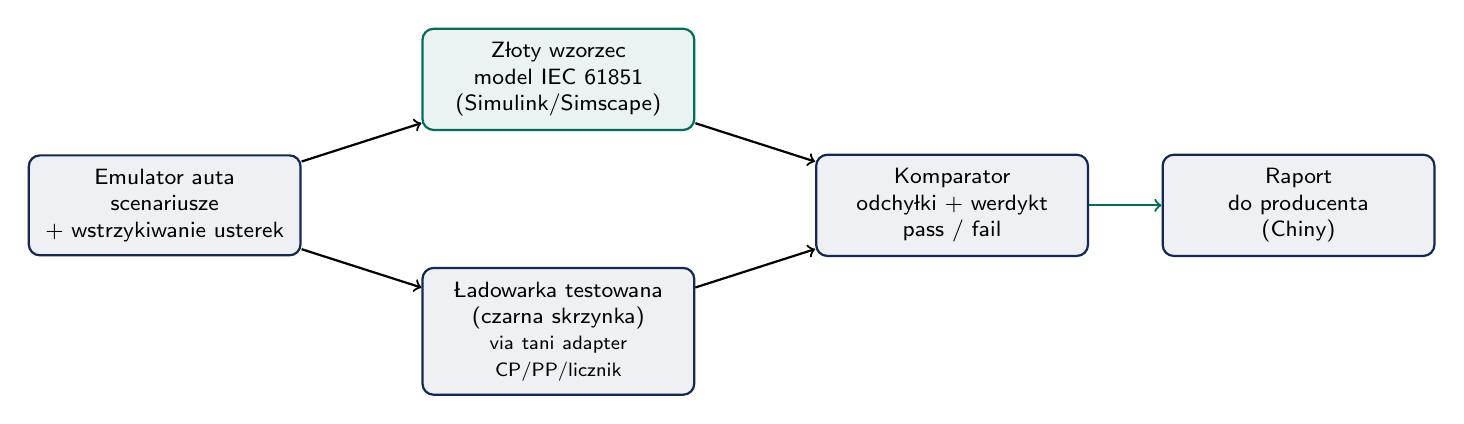
\begin{tikzpicture}[font=\sffamily\footnotesize,
  box/.style={draw=navy,thick,rounded corners,fill=navy!7,align=center,inner sep=5pt,text width=3.1cm,minimum height=1.15cm},
  gold/.style={draw=accent,thick,rounded corners,fill=accent!8,align=center,inner sep=5pt,text width=3.1cm,minimum height=1.15cm}]
  \node[box] (emul) at (0,0) {Emulator auta\\scenariusze\\+ wstrzykiwanie usterek};
  \node[gold] (g) at (5,1.6) {Złoty wzorzec\\model IEC 61851\\(Simulink/Simscape)};
  \node[box] (d) at (5,-1.6) {Ładowarka testowana\\(czarna skrzynka)\\{\scriptsize via tani adapter CP/PP/licznik}};
  \node[box] (c) at (10,0) {Komparator\\odchyłki + werdykt\\pass / fail};
  \node[box] (r) at (14.4,0) {Raport\\do producenta\\(Chiny)};
  \draw[->,thick] (emul) -- (g);
  \draw[->,thick] (emul) -- (d);
  \draw[->,thick] (g) -- (c);
  \draw[->,thick] (d) -- (c);
  \draw[->,thick,accent] (c) -- (r);
\end{tikzpicture}}
\end{center}

\subsection{Czym to się różni od ich obecnego „testera wallboxów''}

Obecny gadżet odpowiada na pytanie \key{„czy w ogóle działa?''} (go/no-go). Mój testbench odpowiada na \key{„jak dokładnie się zachowuje, gdzie odbiega od normy, o ile, i czy nowy firmware tego nie zepsuł?''} --- czyli charakteryzacja, regresja i materiał dowodowy dla producenta.

% ====== SYMULACJA ======
\section{4. Co dokładnie symuluję (Simulink/Simscape) --- i wolne alternatywy}

\subsection{Rdzeń modelu}
\begin{itemize}
  \item \key{Simscape Electrical --- analogowy front-end CP.} Źródło $\pm$12~V/PWM, sieć rezystorów auta (2,74~k$\Omega$ + dioda, dołączany 1,3~k$\Omega$), dzielnik. Widzę realne poziomy 12/9/6~V i kształt PWM --- dowód, że rozumiem warstwę fizyczną, nie tylko logikę.
  \item \key{Stateflow --- maszyna stanów CP.} Dwie sztuki: złoty wzorzec (ładowarka) i emulator auta. Pełen handshake A\ra{}B\ra{}C i z powrotem, z czasami przejść.
  \item \key{Logika prąd/PP.} Przeliczenie wypełnienie~\ra{}~prąd (\,$\times$0,6\,), kodowanie PP, wartości „raportowane'' jak w aplikacji.
\end{itemize}

\subsection{Scenariusz A (kluczowy): weryfikacja licznika energii}
Zadaję znany profil prądu w sesji, liczę \key{prawdziwą energię} (całka mocy po czasie), a model licznika obarczam konfigurowalnym błędem (offset, dryf, kwantyzacja). Testbench wykrywa, gdy \key{raportowane kWh} odbiega ponad tolerancję (np. $\pm$1\%). Efekt: zanim sprzęt trafi do floty, wiem, że licznik nie zawyża faktur --- a jeśli zawyża, mam dokładną liczbę do producenta.

\subsection{Scenariusz B (pokaz integracji): DLB}
Modeluję dom: bezpiecznik główny + zmienne obciążenie domowe + 1--4 ładowarki z DLB. Podnoszę obciążenie i sprawdzam, czy suma prądów \key{nigdy nie przekracza} bezpiecznika i czy ładowarka zdążyła zmniejszyć prąd w wymaganym czasie. Odpinam auto i sprawdzam, czy pozostałe „dobierają'' zwolnioną moc. To wprost dotyka realnych skarg: wybity bezpiecznik / wolne ładowanie.

\subsection{Wolne alternatywy (gdyby brak MATLAB-a)}
\key{Python} (NumPy/SciPy + prosta maszyna stanów, np.\ \texttt{transitions}) do logiki i scenariuszy; \key{Scilab/Xcos} jako darmowy odpowiednik Simulinka; \key{LTspice / ngspice / Falstad} do analogowego obwodu CP. Koncepcja jest niezależna od narzędzia --- MATLAB (licencja uczelniana) tylko ją przyspiesza.

% ====== PLAN 40H ======
\section{5. Plan pracy na ok. 40 h}

\begin{center}
\begin{tabularx}{\linewidth}{@{}c X c@{}}
\toprule
\textbf{Faza} & \textbf{Zakres} & \textbf{h} \\
\midrule
0 & Research normy IEC 61851 (CP/PP, czasy) + lista przypadków testowych & 4 \\
1 & Simscape: analogowy front-end CP (poziomy 12/9/6~V, PWM) & 6 \\
2 & Stateflow: maszyna stanów --- złoty wzorzec + emulator auta & 8 \\
3 & Logika wypełnienie\,\ra\,prąd + kodowanie PP + wartości raportowane & 3 \\
4 & Wstrzykiwanie usterek + komparator + werdykt pass/fail & 7 \\
5 & Scenariusz A: weryfikacja licznika energii (błąd kWh) & 5 \\
6 & Scenariusz B: DLB (bezpiecznik + obciążenia + 2--4 ładowarki) --- elastyczny & 4 \\
7 & Generator raportu do producenta + demo + opis koncepcji & 5 \\
\midrule
\multicolumn{2}{@{}r}{\textbf{Razem}} & \textbf{ok. 42} \\
\bottomrule
\end{tabularx}
\end{center}

Twardy rdzeń (fazy 0--5, 7) to ok. 38~h --- mieści się w budżecie nawet bez fazy DLB. Faza 6 jest „buforem jakości'': robię, jeśli rdzeń idzie sprawnie.

% ====== WARTOSC ======
\section{6. Co to realnie wyłapie (wartość diagnostyczna)}

Każdy przypadek to gotowy, odtwarzalny wpis do raportu dla producenta:

\begin{itemize}
  \item \key{Licznik zawyża/zaniża kWh} ponad tolerancję \ra{} złe rozliczenia floty (uderza w ich główny argument B2B).
  \item \key{Złe wypełnienie PWM} \ra{} ładowarka oferuje inny prąd, niż powinna (za wolno albo ponad bezpiecznik).
  \item \key{Brak reakcji na usterkę} (brak diody, zwarcie CP) zamiast odcięcia \ra{} problem bezpieczeństwa.
  \item \key{Za wolna reakcja DLB} ($>$ wymóg normy) \ra{} ryzyko wybicia bezpiecznika u klienta.
  \item \key{Regresja po nowym firmware:} przypadek, który wcześniej przechodził, teraz nie \ra{} złapane \key{przed} wysyłką do klientów.
\end{itemize}

Zamiast „klient mówi, że coś nie działa'' producent dostaje: \key{który scenariusz, jaka odchyłka, o ile, jak odtworzyć}. To realnie skraca pętlę poprawek z chińską fabryką.

% ====== BUDZET ======
\section{7. Budżet --- kapitał bliski zera}

\begin{center}
\begin{tabularx}{\linewidth}{@{}X r@{}}
\toprule
\textbf{Pozycja} & \textbf{Koszt} \\
\midrule
Symulacja: MATLAB/Simulink/Simscape (licencja uczelniana) & 0 zł \\
\;\; albo wariant darmowy: Python + Scilab/Xcos + LTspice & 0 zł \\
Czas: ok. 40~h pracy własnej & wkład własny \\
\midrule
\multicolumn{2}{@{}l}{\textit{Opcjonalnie --- dopiero do testów realnej ładowarki:}} \\
Tani adapter CP/PP + pomiar (MCU + analog) & 300--500 zł \\
Ładowarka do testów & sprzęt firmy \\
\midrule
\textbf{Koncept + symulacja (deliverable na poniedziałek)} & \textbf{ok. 0 zł kapitału} \\
\bottomrule
\end{tabularx}
\end{center}

To wprost odpowiada na ich strategię „nie topić kapitału'': najpierw tani model, dopiero potem ewentualny sprzęt.

% ====== RYZYKA ======
\section{8. Ryzyka i ograniczenia (uczciwie)}

\begin{itemize}
  \item \key{Model jest tak dobry, jak norma, którą koduję} --- dlatego faza 0 (rzetelne wczytanie IEC 61851) jest krytyczna.
  \item \key{Czarna skrzynka} --- niektóre zachowania wnioskuję z zewnątrz; testbench wskazuje \emph{co} odbiega, nie zawsze \emph{dlaczego} (to już rola producenta).
  \item \key{Adapter dotyka napięcia sieci} --- dlatego wersja symulacyjna jest pełnoprawnym deliverable, a sprzęt to osobny krok z zabezpieczeniami.
  \item \key{To nie certyfikacja} --- narzędzie wspiera diagnostykę i QA, nie zastępuje akredytowanych badań bezpieczeństwa.
\end{itemize}

% ====== PITCH ======
\section{9. Dlaczego to pasuje do firmy (pitch)}

AMPERE POINT zarabia na tym, że \key{lepiej testuje i szybciej adaptuje} cudzy sprzęt niż konkurencja --- „OEM na sterydach''. Mój projekt zamienia ich pętlę „testuj \ra{} zbierz feedback \ra{} zgłoś producentowi'' w \key{powtarzalny, tani, mierzalny proces}: złoty wzorzec łapie odchyłki, regresja pilnuje nowych firmware'ów, a weryfikacja licznika chroni ich główny argument dla flot. Zero kapitału na start, pełna symulacja jako dowód koncepcji --- i jasna ścieżka do wersji sprzętowej, gdy się opłaci.


% ==========================================================
\section{10. Ścieżka realizacji --- od czego zacząć budowę}

Konkretny szkielet modelu: jakie bloki postawić, jakie stany i sygnały, i \key{za co dokładnie każdy element odpowiada}. Pisane tak, by dało się usiąść i zacząć --- nawet przy pierwszym kontakcie z tymi ładowarkami.

\subsection{10.1. Trzy rodzaje klocków (orientacja w minutę)}

\begin{itemize}
  \item \key{Simulink} --- diagram sygnałowy. Bloki (Gain, Sum, Integrator, Lookup) przetwarzają \emph{sygnały} (liczby zmienne w czasie); strzałki mają kierunek. Tu żyje matematyka i logika.
  \item \key{Simscape Electrical} --- symulacja \emph{fizycznego obwodu}. Stawiasz prawdziwe elementy (rezystor, dioda, źródło) i łączysz jak schemat; solver liczy prądy i napięcia z praw Kirchhoffa. Połączenia są dwukierunkowe (fizyczne), nie sygnałowe.
  \item \key{Stateflow} --- maszyna stanów na Simulinku. Rysujesz stany (prostokąty) i przejścia (strzałki z warunkami); w każdym kroku czasu sprawdza warunki i reaguje. Tu żyje „mózg'' ładowarki i auta.
  \item \key{Mostki} --- \texttt{Simulink-PS Converter} i \texttt{PS-Simulink Converter} przekładają sygnał Simulinka na wielkość fizyczną Simscape'a i odwrotnie. \key{Solver Configuration} to obowiązkowy blok każdego obwodu Simscape.
\end{itemize}

\subsection{10.2. Architektura modelu i sygnały}

Sześć podsystemów; strzałki to sygnały płynące między nimi. Emulator auta i wzorzec spotykają się na \key{warstwie fizycznej CP} (to „kabel''), a osobno na \key{torze mocy} (to „prąd ładowania'').

\begin{center}
\resizebox{\linewidth}{!}{%
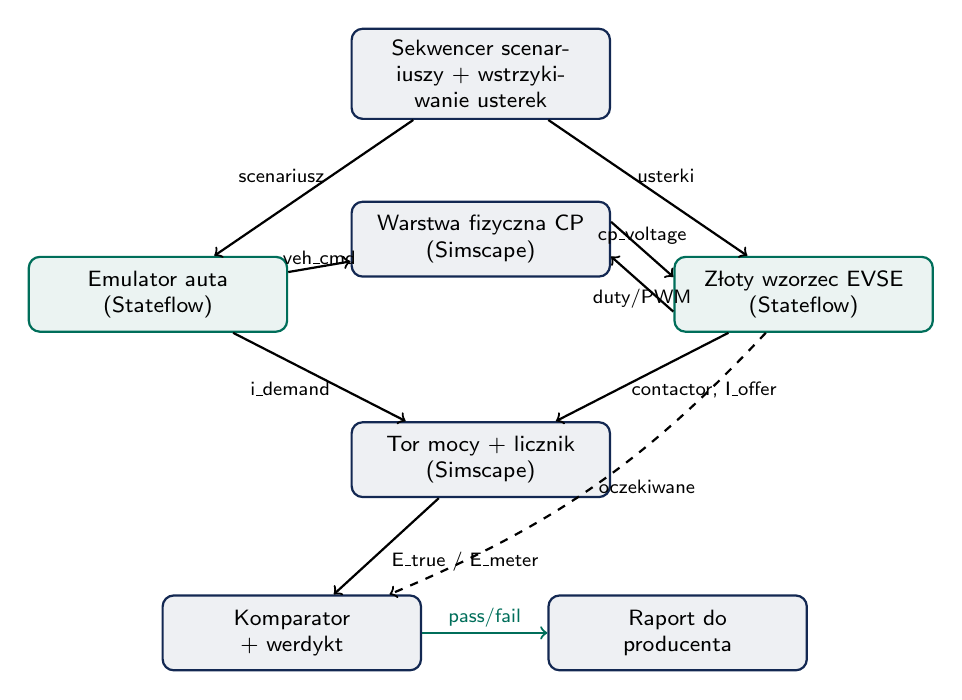
\begin{tikzpicture}[font=\sffamily\footnotesize,
  b/.style={draw=navy,thick,rounded corners,fill=navy!7,align=center,inner sep=4pt,text width=3.0cm,minimum height=0.95cm},
  sf/.style={draw=accent,thick,rounded corners,fill=accent!8,align=center,inner sep=4pt,text width=3.0cm,minimum height=0.95cm},
  sig/.style={font=\sffamily\scriptsize,inner sep=1.5pt}]
  \node[b]  (seq)  at (4.1,7.4) {Sekwencer scenariuszy + wstrzykiwanie usterek};
  \node[sf] (emul) at (0,4.6) {Emulator auta\\(Stateflow)};
  \node[b]  (cpp)  at (4.1,5.3) {Warstwa fizyczna CP\\(Simscape)};
  \node[b]  (pwr)  at (4.1,2.5) {Tor mocy + licznik\\(Simscape)};
  \node[sf] (evse) at (8.2,4.6) {Złoty wzorzec EVSE\\(Stateflow)};
  \node[b]  (cmp)  at (1.7,0.3) {Komparator\\+ werdykt};
  \node[b]  (rep)  at (6.6,0.3) {Raport do\\producenta};
  \draw[->,thick] (seq) -- (emul) node[sig,midway,above left,xshift=2mm]{scenariusz};
  \draw[->,thick] (seq) -- (evse) node[sig,midway,above right,xshift=-2mm]{usterki};
  \draw[->,thick] (emul) -- (cpp) node[sig,midway,above,yshift=-1pt]{veh\_cmd};
  \draw[->,thick] ([yshift=-2.2mm]evse.west) -- ([yshift=-2.2mm]cpp.east) node[sig,midway,below]{duty/PWM};
  \draw[->,thick] ([yshift=2.2mm]cpp.east) -- ([yshift=2.2mm]evse.west) node[sig,midway,above]{cp\_voltage};
  \draw[->,thick] (emul) -- (pwr) node[sig,midway,below left,xshift=2mm]{i\_demand};
  \draw[->,thick] (evse) -- (pwr) node[sig,midway,below right,xshift=-2mm]{contactor, I\_offer};
  \draw[->,thick] (pwr) -- (cmp) node[sig,midway,below right]{E\_true / E\_meter};
  \draw[->,thick,dashed] (evse) to[bend left=12] node[sig,midway,right]{oczekiwane} (cmp);
  \draw[->,thick,accent] (cmp) -- (rep) node[sig,midway,above]{pass/fail};
\end{tikzpicture}}
\end{center}

\begin{center}
\begin{tabularx}{\linewidth}{@{}l l X l@{}}
\toprule
\textbf{Sygnał} & \textbf{Jedn.} & \textbf{Znaczenie} & \textbf{Z \ra{} do} \\
\midrule
\texttt{cp\_voltage} & V & napięcie linii Control Pilot & warstwa CP \ra{} wzorzec \\
\texttt{duty} & \% & wypełnienie PWM (koduje prąd) & wzorzec \ra{} warstwa CP \\
\texttt{veh\_cmd} & --- & które rezystory/dioda wpięte & emulator \ra{} warstwa CP \\
\texttt{I\_offer} & A & prąd oferowany autu & wzorzec \ra{} tor mocy \\
\texttt{i\_demand} & A & prąd, jaki auto chce pobrać & emulator \ra{} tor mocy \\
\texttt{contactor\_cmd} & 0/1 & zamknięcie stycznika mocy & wzorzec \ra{} tor mocy \\
\texttt{pp\_resistance} & $\Omega$ & kod kabla (Proximity Pilot) & emulator \ra{} wzorzec \\
\texttt{E\_true / E\_meter} & kWh & energia prawdziwa / zliczona & tor mocy \ra{} komparator \\
\texttt{verdict} & pass/fail & wynik testu + odchyłka & komparator \ra{} raport \\
\bottomrule
\end{tabularx}
\end{center}

\subsection{10.3. Faza 1 --- Warstwa fizyczna CP (Simscape Electrical)}

\key{Co ma robić:} odtworzyć realne napięcia Control Pilot (12 / 9 / 6~V) i sygnał PWM, żebyś widział warstwę fizyczną na wykresie (Scope), nie tylko liczby.

\key{Bloki i ich rola:}
\begin{itemize}
  \item \key{Controlled Voltage Source} --- generuje falę CP; steruje nim sygnał PWM $\pm$12~V z Simulinka (przez \texttt{Simulink-PS Converter}). To „nadajnik'' ładowarki.
  \item \key{Pulse Generator} (Simulink) --- 1~kHz, wypełnienie ustawiane sygnałem \texttt{duty}. Odpowiada za zakodowanie prądu w szerokości impulsu.
  \item \key{Resistor R1 = 1~k$\Omega$} (strona ładowarki, szeregowo) --- rezystor pilota; z siecią auta tworzy \key{dzielnik napięcia} ustalający poziom CP.
  \item \key{Resistor R2 = 2,74~k$\Omega$} + \key{Diode} (strona auta) --- po wpięciu dzielnik daje ok.\ 9~V = stan~B. Dioda jest po to, by ładowarka „widziała'', że to prawdziwe auto (rezystor bez diody = usterka).
  \item \key{Resistor R3 = 1,3~k$\Omega$} + \key{Ideal Switch} --- dołączany równolegle do R2 (przełącznik sterowany przez emulator). Obniża poziom do ok.\ 6~V = stan~C (auto gotowe).
  \item \key{Voltage Sensor} + \key{PS-Simulink Converter} --- mierzy napięcie CP i oddaje je do Simulinka jako \texttt{cp\_voltage}. To „oczy'' obu maszyn stanów.
  \item \key{Solver Configuration} + \key{Electrical Reference} (masa = PE) --- obowiązkowe dla obwodu.
\end{itemize}

\key{Skąd te wartości:} dzielnik 1~k$\Omega$ (ładowarka) z 2,74~k$\Omega$ (auto) daje $12\cdot 2{,}74/(1{+}2{,}74)\approx 9$~V; po dołączeniu 1,3~k$\Omega$ równolegle opór auta spada do ok.\ 0,88~k$\Omega$, a napięcie do ok.\ 6~V. Stąd progi 9/6~V.

\key{Kamień milowy:} na Scope widzisz prostokąt $\pm$12~V, a poziom górny przeskakuje 9~V\,\ra\,6~V, gdy emulator przełącza stan B\,\ra\,C.

\subsection{10.4. Faza 2 --- Maszyny stanów (Stateflow)}

Dwie karty: jedna udaje auto, druga to wzorzec ładowarki.

\subsubsection{Karta „Emulator auta''}
Steruje stroną auta i prowadzi scenariusz. \key{Stany:} \texttt{A\_Unplugged} \ra{} \texttt{B\_Connected} \ra{} \texttt{C\_Ready} (+ \texttt{Fault}). \key{Wyjścia:} \texttt{veh\_cmd} (które rezystory/diodę wpiąć), \texttt{i\_demand} (ile prądu auto chce w stanie C). \key{Wejścia:} komendy ze sekwencera.

\subsubsection{Karta „Złoty wzorzec EVSE''}
Wzorcowa logika ładowarki wg IEC 61851. \key{Wejścia:} \texttt{cp\_voltage} (czyta poziom \ra{} wnioskuje stan auta), \texttt{pp\_resistance}, limity prądu. \key{Stany:} \texttt{Idle} (stałe $+12$~V, bez PWM) \ra{} \texttt{Detected} (wykrył 9~V \ra{} włącza PWM o wypełnieniu = prąd/0,6) \ra{} \texttt{Charging} (wykrył 6~V \ra{} zamyka stycznik) \ra{} \texttt{Fault} (nielegalny CP \ra{} otwiera stycznik). \key{Wyjścia:} \texttt{duty}, \texttt{contactor\_cmd}. \key{Wymóg czasowy:} po komendzie zmniejszenia prądu (DLB) wypełnienie zmienia się w ciągu kilku sekund --- to później testujemy.

\key{Pętla:} wzorzec ustawia \texttt{duty} \ra{} Pulse Generator (warstwa CP) \ra{} \texttt{cp\_voltage} \ra{} wraca do obu kart. To zamknięta pętla sterowania, jak w realu.

\key{Kamień milowy:} uruchamiasz symulację i widzisz pełny handshake A\,\ra\,B\,\ra\,C\,\ra\,A oraz \texttt{duty}/\texttt{contactor\_cmd} reagujące zgodnie z normą.

\subsection{10.5. Faza 3 --- Prąd, PP i wartości raportowane}

\key{Co robi:} zamienia logikę na konkretne liczby prądu i pilnuje limitów.
\begin{itemize}
  \item \key{Gain $\times$0,6} + \key{Saturation} (6--80~A) --- przelicza wypełnienie na prąd i ogranicza do zakresu. (Można 1-D Lookup Table, by ująć regułę 10--85\% i wyjątek 5\% = komunikacja cyfrowa.)
  \item \key{1-D Lookup Table (PP)} --- mapuje rezystancję PP na obciążalność kabla (np.\ 1,5~k$\Omega$\,\ra\,13~A, 680~$\Omega$\,\ra\,20~A, 220~$\Omega$\,\ra\,32~A).
  \item \key{MinMax} --- prąd oferowany = minimum z: limit instalacji, limit kabla (PP), limit DLB. Tak realnie ładowarka wybiera prąd.
  \item \key{Podsystem „wartości raportowane''} --- liczy, co pokazałby wyświetlacz/aplikacja (prąd, napięcie, energia), by porównać raport z rzeczywistością.
\end{itemize}

\subsection{10.6. Faza 4 --- Wstrzykiwanie usterek i komparator}

\key{Wstrzykiwanie usterek} --- przełączniki/flagi (panel parametrów lub Signal Builder) celowo psujące model:
\begin{itemize}
  \item \texttt{no\_diode} --- wyłącza diodę (wzorzec ma wykryć i przejść w \texttt{Fault}).
  \item \texttt{cp\_short} --- wymusza \texttt{cp\_voltage}=0 (zwarcie do PE) \ra{} stan~E.
  \item \texttt{duty\_error} --- offset wypełnienia (blok \key{Sum}); firmware oferuje zły prąd.
  \item \texttt{slow\_response} --- \key{Transport Delay} na zmianie \texttt{duty}; za wolna reakcja na DLB.
  \item \texttt{meter\_error} --- \key{Gain}/offset na liczniku energii.
\end{itemize}

\key{Komparator} --- porównuje obiekt z wzorcem i wystawia werdykt:
\begin{itemize}
  \item prąd oferowany vs oczekiwany: \key{Sum} \ra{} \key{Abs} \ra{} \key{Compare To Constant} (tolerancja).
  \item czas reakcji vs próg: timer mierzy odstęp komenda\,\ra\,zmiana \texttt{duty}.
  \item błąd licznika vs tolerancja; legalność przejść stanów.
\end{itemize}
Bloki: \key{Relational Operator}, \key{Compare To Constant}, \key{Logical Operator}, (opcjonalnie \key{Assertion}). Wyjście: \texttt{verdict} + zmierzone odchyłki.

\subsection{10.7. Faza 5 --- Tor mocy i weryfikacja licznika}

\key{Co robi:} sprawdza, czy zliczona energia (kWh) zgadza się z prawdą --- ich filar dla flot.
\begin{itemize}
  \item \key{AC Voltage Source} (230/400~V) --- sieć.
  \item \key{Controlled Current Source} (lub \key{Variable Resistor}) --- udaje ładowarkę pokładową auta pobierającą \texttt{i\_demand} (do \texttt{I\_offer}).
  \item \key{Current Sensor} + \key{Voltage Sensor} --- mierzą prąd i napięcie.
  \item \key{Product} ($P=U\cdot I$) \ra{} \key{Integrator} ($\int P\,dt$) \ra{} \key{Gain 1/3600} \ra{} \texttt{E\_true} [kWh]. Integrator sumuje pole pod krzywą mocy = energia.
  \item \key{Model licznika}: ta sama całka przepuszczona przez \texttt{meter\_error} (gain/offset/kwantyzacja) \ra{} \texttt{E\_meter}.
  \item \key{Komparator}: błąd~\% $=(E_{meter}-E_{true})/E_{true}\cdot 100$ \ra{} Compare to $\pm$1\% \ra{} pass/fail.
\end{itemize}

\subsection{10.8. Faza 6 --- Scenariusz DLB}

\key{Co robi:} sprawdza, czy ładowarki dzielą moc tak, by nie wybić bezpiecznika.
\begin{itemize}
  \item \key{Signal Builder} --- profil obciążenia domowego w czasie (rośnie/maleje).
  \item \key{1--4 gałęzie ładowarek} --- każda to sterowane źródło prądu ustawiane jej \texttt{I\_offer}.
  \item \key{Sum} --- prąd całkowity = dom + suma ładowarek.
  \item \key{Kontroler DLB} (w karcie wzorca): gdy suma zbliża się do limitu bezpiecznika \ra{} zmniejsza \texttt{duty} ładowarek; po odpięciu auta \ra{} dobiera wolną moc.
  \item \key{Compare To Constant} + \key{Assertion} --- pilnują, że prąd całkowity $\le$ bezpiecznik \emph{zawsze}; timer mierzy czas reakcji.
\end{itemize}

\subsection{10.9. Faza 7 --- Sekwencer scenariuszy i raport}

\begin{itemize}
  \item \key{Test Sequence} (Simulink Test) / karta Stateflow / skrypt MATLAB --- uruchamia scenariusze po kolei, ustawia flagi usterek, zbiera werdykty.
  \item \key{To Workspace / Simulation Data Inspector} --- loguje sygnały.
  \item \key{Skrypt raportu} --- buduje tabelę: scenariusz, odchyłka, wielkość, jak odtworzyć \ra{} eksport do PDF/CSV. To artefakt, który jedzie do producenta.
\end{itemize}

\subsection{10.10. Wariant w pełni darmowy (gdyby brak MATLAB-a)}

Ta sama koncepcja, mapowanie 1:1:
\begin{itemize}
  \item \key{Logika i maszyny stanów} \ra{} \key{Python} (biblioteka \texttt{transitions} lub własny FSM; \texttt{numpy/scipy} do całek i sygnałów).
  \item \key{Obwód CP} \ra{} \key{LTspice} / \key{ngspice} / \key{Falstad} (ten sam dzielnik R1/R2/R3 + dioda) --- weryfikujesz poziomy 9/6~V.
  \item \key{Diagram blokowy} \ra{} \key{Scilab/Xcos} (darmowy odpowiednik Simulinka).
  \item \key{Raport} \ra{} \texttt{pandas} \ra{} CSV/Markdown/PDF.
\end{itemize}

\subsection{10.11. Kolejność budowy i pierwszy kamień milowy}

Buduj \key{od dołu do góry}, mały działający kawałek na raz:
\begin{enumerate}
  \item Obwód CP w Simscape \ra{} zobacz 9~V/6~V (pół dnia). \key{To Twój pierwszy kamień milowy} --- gdy go masz, reszta to nadbudowa.
  \item Dołóż dwie karty Stateflow \ra{} pełny handshake.
  \item Dołóż prąd/PP, potem licznik (faza 5).
  \item Dołóż wstrzykiwanie usterek + komparator \ra{} pierwszy automatyczny pass/fail.
  \item Na końcu DLB oraz sekwencer + raport.
\end{enumerate}
Po każdym kroku masz coś, co działa i co możesz pokazać --- a nie wielki model, który „nie wiadomo czemu nie rusza''.

\end{document}
